\documentclass[aspectratio=169,11pt]{beamer}
\usepackage[utf8]{inputenc}
\usepackage[T1]{fontenc}
\usepackage[spanish,es-noshorthands,es-nodecimaldot]{babel}
\usepackage{booktabs}
\usetheme{default}
\usecolortheme{dove}
\setbeamertemplate{navigation symbols}{}
\setbeamertemplate{footline}[frame number]
\definecolor{navy}{HTML}{1C2F54}
\setbeamercolor{frametitle}{fg=navy}
\setbeamercolor{title}{fg=navy}
\setbeamerfont{frametitle}{series=\bfseries}
\graphicspath{{figures/}}

\title{Predicción del nivel relativo de comisiones\\del siguiente bloque de Bitcoin}
\subtitle{Proyecto final --- Etapa 2 (modelado, evaluación y discusión)}
\author{Carlos Ordinola \and Nayeli Guerrero \and Adriana Alvarado}
\institute{Machine Learning (CS3061) --- UTEC 2026-2}
\date{}

\begin{document}

\begin{frame}
\centering

\includegraphics[height=1.2cm]{utec_logo.png}\par\vspace{0.4cm}
\titlepage
\end{frame}

% ---------------- Carlos: problema, datos y baselines (≈3 min) ----------------
\begin{frame}{El problema}
\begin{itemize}
\item El espacio de cada bloque es limitado: las transacciones compiten pagando comisiones.
\item Pagar poco implica esperar horas; pagar de más es un costo irrecuperable.
\item \textbf{Tarea:} dado el bloque $t$, predecir si la tasa mediana del bloque $t+1$ superará el percentil 75 de las últimas 1008 tasas (una semana).
\[ y_t = 1 \iff f_{t+1} > P_{75}(f_{t-1007},\dots,f_t) \]
\item \textbf{Métrica principal:} F1 de la clase alta. Referencia: \textbf{persistencia} (``el siguiente bloque será como el actual'').
\item \textbf{Hipótesis:} H1 la tasa reciente domina; H2 la actividad de la red aporta poco; H3 el modelo empeora con alta volatilidad.
\end{itemize}
\end{frame}

\begin{frame}{Datos y decisiones de P1}
\begin{columns}[T]
\column{0.5\textwidth}
\small
\begin{itemize}
\item 810\,909 bloques (Kaggle, 2009--2023), 13 variables por bloque.
\item Desde 2016 los bloques se llenan y aparece la competencia por comisión $\Rightarrow$ estudio desde 2016.
\item Umbral fijo: 0.32\,\% de positivos en validación. Umbral móvil: 24.7 / 21.5 / 24.9\,\%.
\item Partición cronológica 70/15/15: 418\,720 ejemplos.
\end{itemize}
\column{0.5\textwidth}
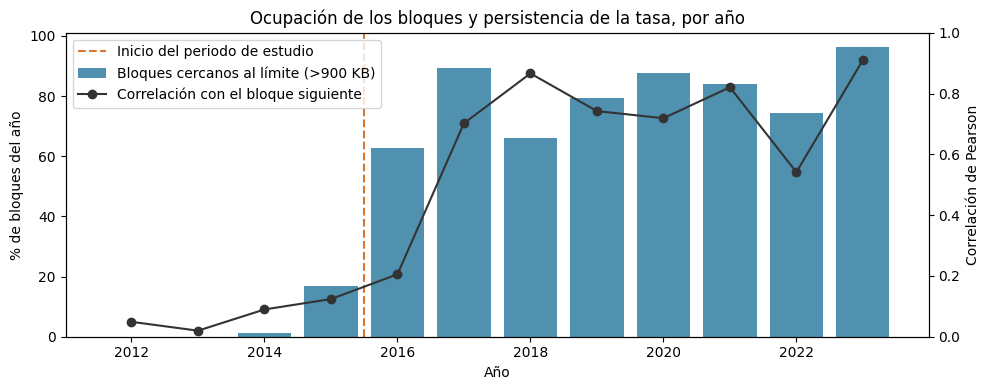
\includegraphics[width=\textwidth]{ocupacion_por_anio.png}
\end{columns}
\end{frame}

\begin{frame}{Referencias: persistencia y regresión logística}
\begin{columns}[T]
\column{0.48\textwidth}
\small
\begin{itemize}
\item Si el bloque actual es ``alto'', el siguiente también lo es el 52.8\,\% de las veces (15.5\,\% si no).
\item Logística L2 con 22 variables, umbral ajustado en validación.
\item \textbf{En prueba, la persistencia gana:} F1 0.576 frente a 0.570.
\item La logística sí discrimina (AP 0.617 frente a 0.249 de tasa base), pero no supera la inercia del mercado.
\end{itemize}
\column{0.52\textwidth}
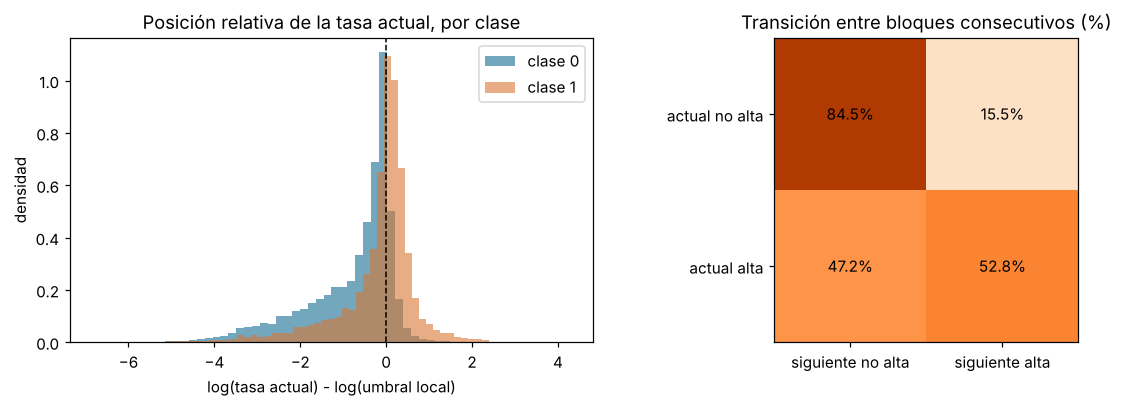
\includegraphics[width=\textwidth]{eda_posicion_relativa.png}
\end{columns}
\end{frame}

% ---------------- Nayeli: ensambles y diseño experimental (≈3 min) ----------------
\begin{frame}{Modelos de ensamble y diseño experimental}
\begin{itemize}
\item \textbf{Random Forest} (bagging) e \textbf{HistGradientBoosting} (boosting) con 33 variables causales: rezagos, medias y desviaciones móviles de la tasa, actividad y calendario.
\item Tres folds de \textbf{ventana expansiva} dentro de entrenamiento, con \textit{gap} de 1008 bloques.
\item Búsqueda acotada: 3 configuraciones por familia; umbral de decisión elegido con predicciones fuera de fold.
\item Reajuste final y una sola evaluación en validación. El test se reserva.
\end{itemize}
\end{frame}

\begin{frame}{Resultados}
\begin{columns}[T]
\column{0.52\textwidth}
\small
\begin{tabular}{lccc}
\toprule
Método & F1 val. & AP val. & F1 prueba \\
\midrule
Persistencia & 0.540 & -- & 0.576 \\
Logística & 0.557 & 0.593 & 0.570 \\
Random Forest & 0.564 & 0.623 & pend. \\
HGB & 0.571 & 0.630 & pend. \\
\bottomrule
\end{tabular}
\vspace{0.3cm}
\begin{itemize}
\item Los árboles superan a las referencias en validación: +0.03 de F1 frente a la persistencia y +0.04 de AP frente a la logística.
\end{itemize}
\column{0.48\textwidth}
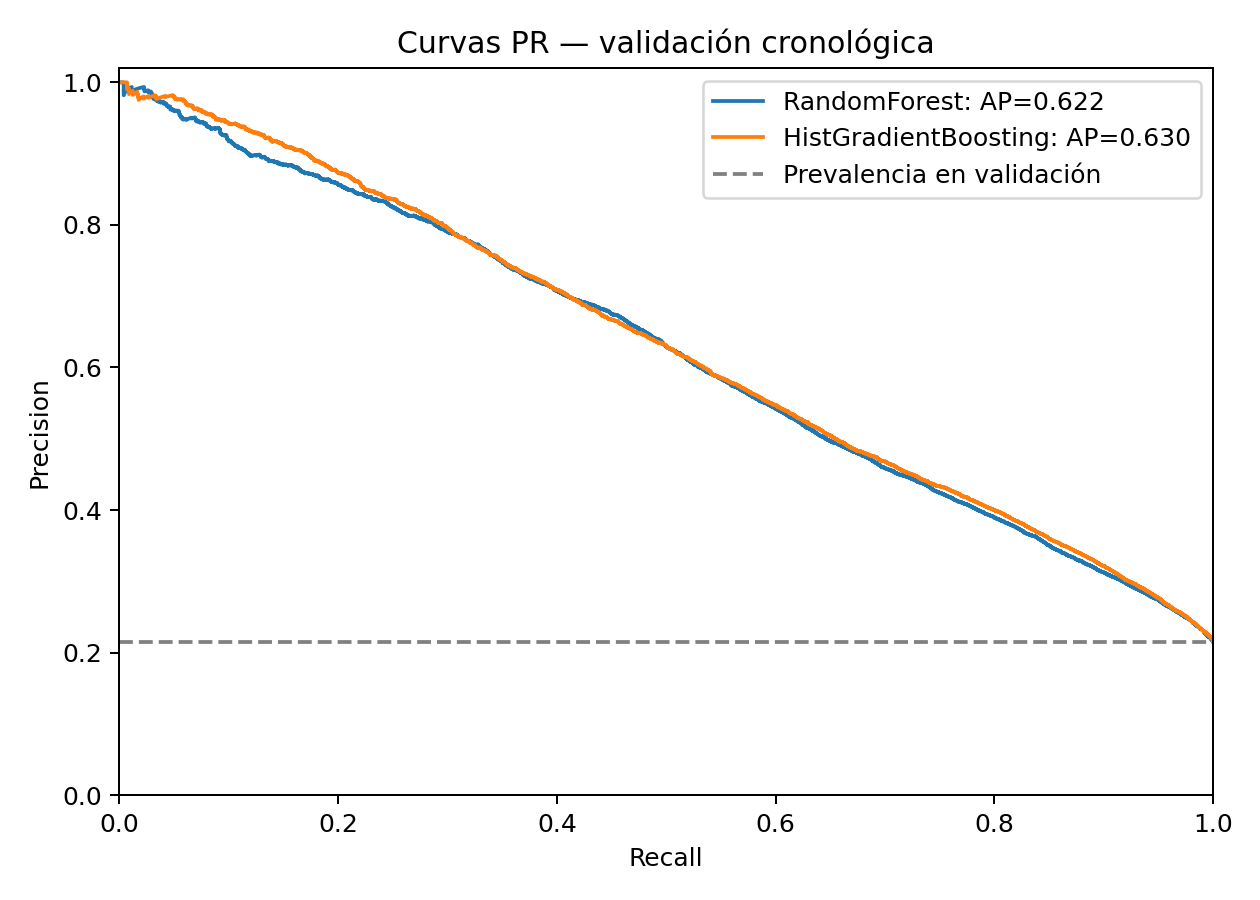
\includegraphics[width=\textwidth]{curvas_pr.png}
\end{columns}
\end{frame}

% ---------------- Adriana: ablation, errores y conclusiones (≈4 min) ----------------
\begin{frame}{Ablation: ¿qué información aporta cada grupo?}
\begin{columns}[T]
\column{0.42\textwidth}
\small
Mismo HGB, mismos folds, cuatro conjuntos de variables:
\begin{itemize}
\item \textbf{A0} tasa actual (3): igual a la persistencia.
\item \textbf{A} + historia de comisiones: \textbf{+0.084 AP}.
\item \textbf{B} + actividad de la red: +0.012 AP.
\item \textbf{C} + calendario: sin mejora.
\end{itemize}
IC 95\,\% por \textit{bootstrap} de bloques semanales.\\[0.2cm]
$\Rightarrow$ \textbf{H1 y H2 se confirman.}
\column{0.58\textwidth}
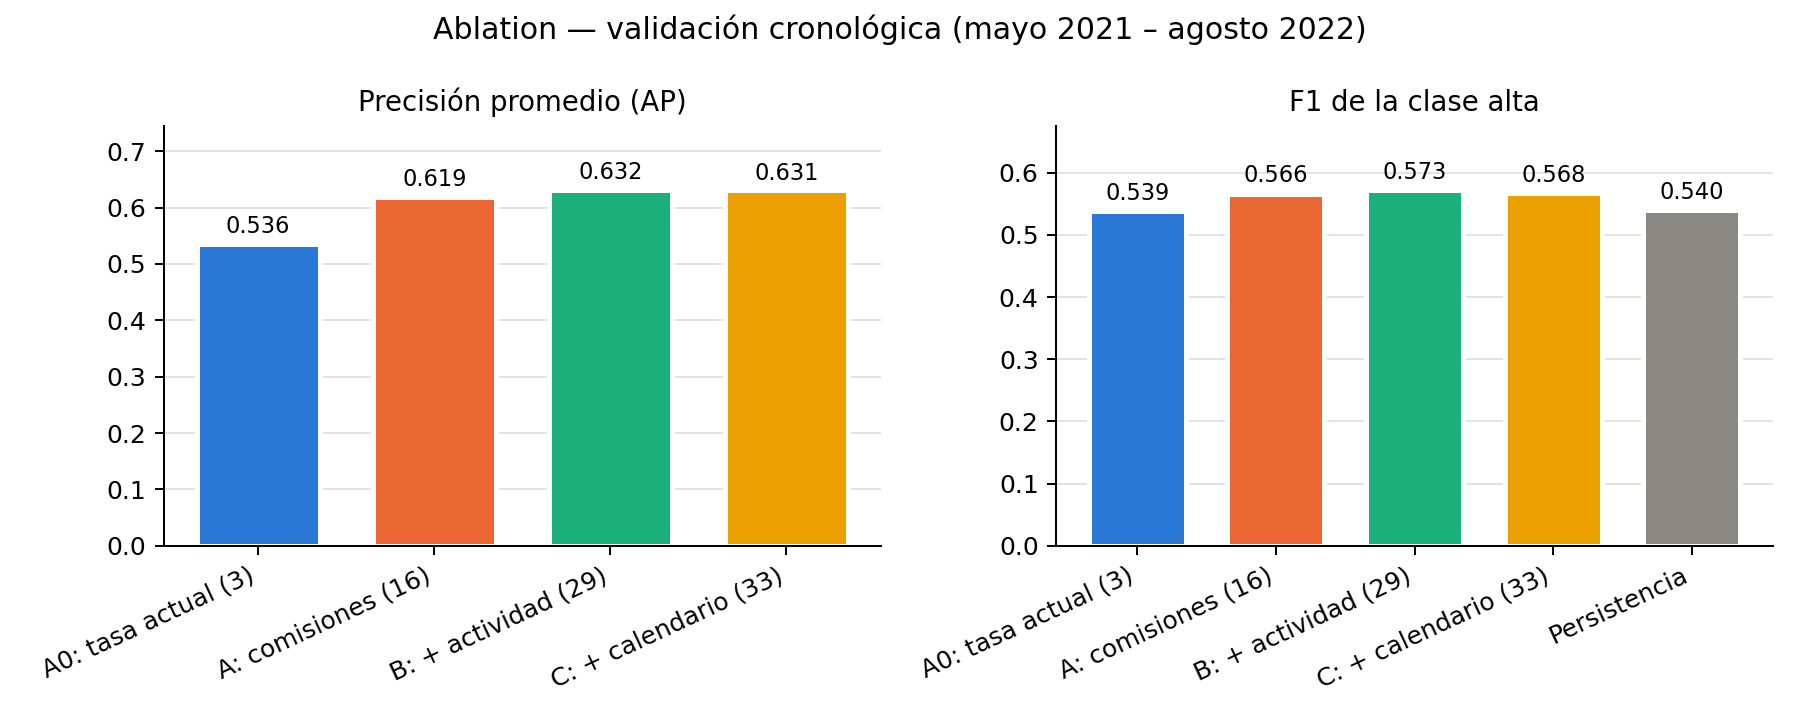
\includegraphics[width=\textwidth]{ablation_validacion.png}
\end{columns}
\end{frame}

\begin{frame}{¿Dónde se equivocan los modelos?}
\begin{columns}[T]
\column{0.42\textwidth}
\small
\begin{itemize}
\item Un episodio de comisión alta dura \textbf{2.2 bloques} en promedio; el 20\,\% de los bloques es un cambio de clase.
\item El modelo anticipa el 39\,\% de los finales, pero solo el \textbf{14\,\% de los inicios}.
\item El inicio es demanda nueva en el \textit{mempool}, que el dataset no registra.
\item Volatilidad alta: F1 0.548 frente a 0.566--0.575 $\Rightarrow$ \textbf{H3 parcial}.
\end{itemize}
\column{0.58\textwidth}
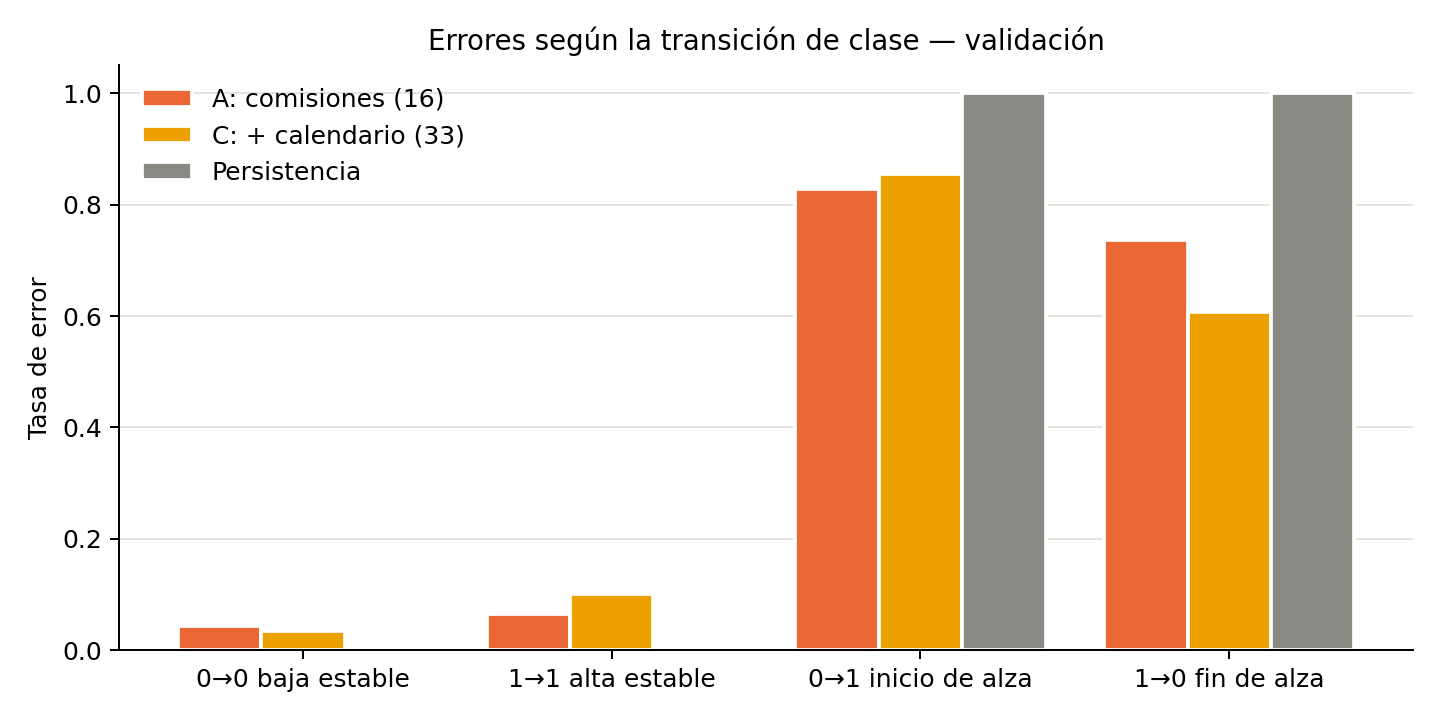
\includegraphics[width=\textwidth]{errores_por_transicion.png}
\end{columns}
\end{frame}

\begin{frame}{Los errores se concentran cerca del umbral}
\centering
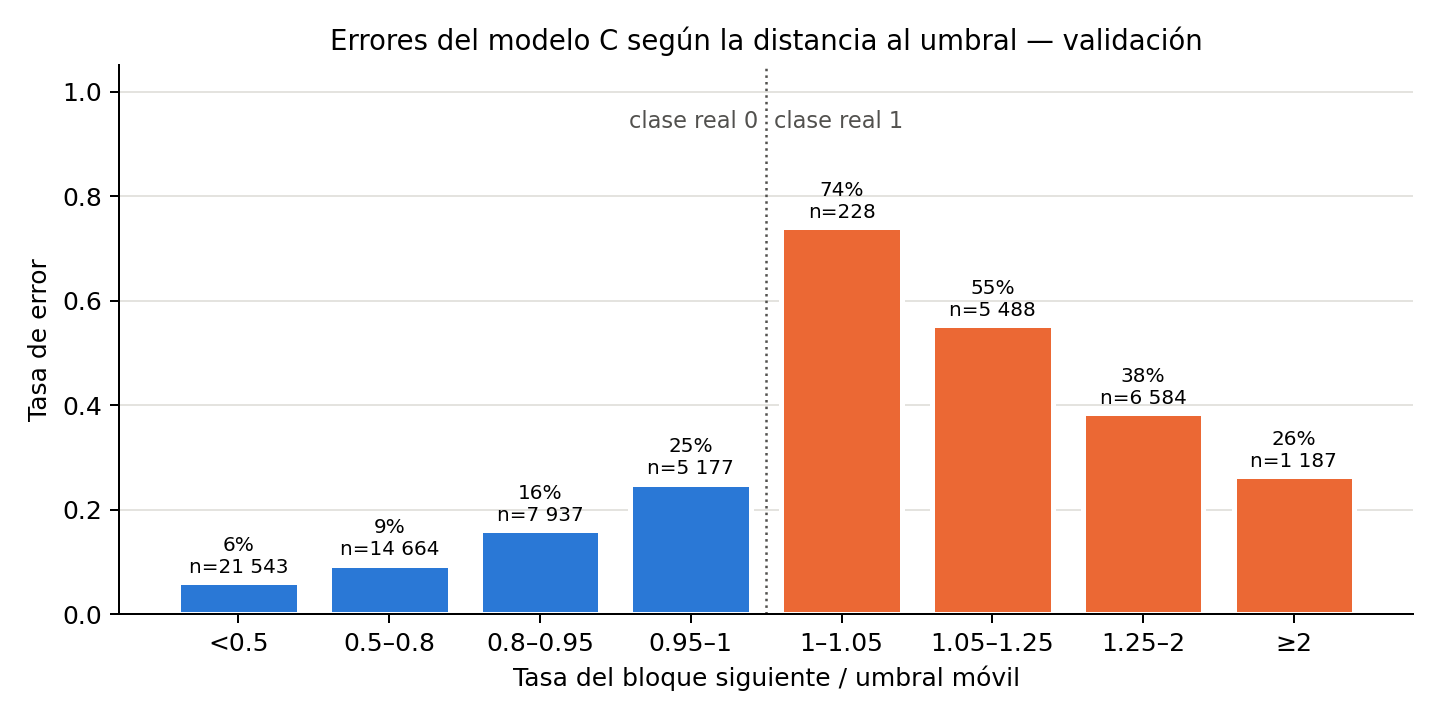
\includegraphics[height=0.62\textheight]{errores_por_margen.png}\par
\small Cuando el bloque siguiente supera el umbral por menos del 5\,\%, el error es del 74\,\%: la frontera de la clase pone un techo al rendimiento.
\end{frame}

\begin{frame}{Limitaciones y ética}
\begin{itemize}
\item Sin datos del \textit{mempool}; solo transacciones confirmadas y agregadas por bloque.
\item Bloques consecutivos dependientes: intervalos aproximados.
\item Logística y árboles usan conjuntos de variables distintos (22 y 33).
\item Validación con pocos episodios de alta volatilidad; periodo 2016--2023.
\item \textbf{Ética:} una predicción que falla al inicio de la congestión podría inducir malas decisiones; debe comunicarse su incertidumbre y no presentarse como estimador completo.
\end{itemize}
\end{frame}

\begin{frame}{Conclusiones}
\begin{itemize}
\item La persistencia es una referencia difícil: la logística no la supera en prueba.
\item El valor predictivo está en la \textbf{historia reciente de las comisiones}, no en el estado instantáneo ni en el volumen de la red.
\item El límite principal no es el algoritmo, sino la \textbf{información disponible}.
\item \textbf{Trabajo futuro:} datos del \textit{mempool}, detectar el inicio de la congestión como tarea propia, horizontes mayores y clases con margen alrededor del umbral.
\end{itemize}
\vspace{0.4cm}
\centering\small Repositorio: \url{github.com/naye-gg/bitcoin-block-fee-classification_ML_project}
\end{frame}

\end{document}
